%Template
%Copyright (C) 2019  Patrick Diehl
%
%This program is free software: you can redistribute it and/or modify
%it under the terms of the GNU General Public License as published by
%the Free Software Foundation, either version 3 of the License, or
%(at your option) any later version.

%This program is distributed in the hope that it will be useful,
%but WITHOUT ANY WARRANTY; without even the implied warranty of
%MERCHANTABILITY or FITNESS FOR A PARTICULAR PURPOSE.  See the
%GNU General Public License for more details.

%You should have received a copy of the GNU General Public License
%along with this program.  If not, see <http://www.gnu.org/licenses/>.
\providecommand\classoption{12pt}
\documentclass[\classoption]{beamer}

 \newcommand{\orcid}[1]{\href{https://orcid.org/#1}{
\includegraphics[height=10pt]{images/orcid}}}

\mode<beamer>{
\usepackage{template/dbt}
\setbeamercolor{mycolor}{fg=background,bg=background}
}

\mode<handout>{%
	\usepackage{handoutWithNotes} 
    \pgfpagesuselayout{4 on 1 with notes}[letterpaper] 
    \setbeameroption{show notes}
    \usetheme{default}
}

\beamertemplatenavigationsymbolsempty
% usepackage

\definecolor{azure}{rgb}{0.0, 0.5, 1.0}
\definecolor{awesome}{rgb}{1.0, 0.13, 0.32}

\usepackage{lstautodedent}
% lstlisting
\lstset{
    language=C,
    basicstyle=\footnotesize\ttfamily,
    keywordstyle=\color{awesome},
    showspaces=false,
    showstringspaces=false,
    commentstyle=\color{azure}\emph,
	autodedent
    %frame=single,
    %rulecolor=\color{comments},
    %rulesepcolor=\color{comments},
    %backgroundcolor = \color{lightgray}
}

\lstset{inputpath=./ParallelComputationMathExamples/}

\usepackage[
    type={CC},
    modifier={by-nc-nd},
    version={4.0},
]{doclicense} 

\usepackage{ifxetex}

\ifxetex
\usepackage{fontspec}
\setmainfont{Raleway}
\fi

\ifluatex
\usepackage{fontspec}
\setmainfont{Raleway}
\fi

\usepackage{xfrac}

\usepackage{tikz}

\newcommand{\courseurl}[0]{https://www.cct.lsu.edu/\string~pdiehl/teaching/2021/4997/}
\newcommand{\coursetimeline}[0]{https://www.cct.lsu.edu/~pdiehl/teaching/2021/4997/timeline.pdf}
\newcommand{\coursesyllabus}[0]{https://www.cct.lsu.edu/~pdiehl/teaching/2021/4997/syllabus.pdf}
\newcommand{\coursename}[0]{Math 4997-3}
\newcommand{\coursemailinglist}[0]{https://mail.cct.lsu.edu/mailman/listinfo/par4997}
\newcommand{\coursesemester}{Fall 2021}








% frame slide
\title{\coursename}
\subtitle{Lecture 12: One-dimensional heat equation}

\author{\tiny Patrick Diehl \orcid{0000-0003-3922-8419}}
%\institute {
%    \href{}{\tt \scriptsize \today}
%}
\date {
 \tiny \url{\courseurl}
\vspace{2cm}
\doclicenseThis  
  
}



\usepackage{ifxetex}

\ifxetex
\usepackage{fontspec}
\setmainfont{Raleway}
\fi

\ifluatex
\usepackage{fontspec}
\setmainfont{Raleway}
\fi


\begin{document} {
    \setbeamertemplate{footline}{}
    \frame {
        \titlepage
    }
}

\frame{

\tableofcontents

}

\AtBeginSection[]{
  \begin{frame}
  \vfill
  \centering
  \begin{beamercolorbox}[sep=8pt,center,shadow=true,rounded=true]{title}
    \usebeamerfont{title}\insertsectionhead\par%
  \end{beamercolorbox}
  \vfill
  \end{frame}
}

%%%%%%%%%%%%%%%%%%%%%%%%%%%%%%%%%%%%%%%%%%%%%%%%%%%%%%%%%%%%%%%%%%%%%%%%%%%%%%
\section{Reminder}
%%%%%%%%%%%%%%%%%%%%%%%%%%%%%%%%%%%%%%%%%%%%%%%%%%%%%%%%%%%%%%%%%%%%%%%%%%%%%%
\begin{frame}{Lecture 12}
\begin{block}{What you should know from last lecture}
\begin{itemize}
\item What is HPX
\item Asynchronous programming using HPX
\item Shared memory parallelism using HPX
\end{itemize}
\end{block}
\end{frame}

%%%%%%%%%%%%%%%%%%%%%%%%%%%%%%%%%%%%%%%%%%%%%%%%%%%%%%%%%%%%%%%%%%%%%%%%%%%%%%
\section{Heat equation}
%%%%%%%%%%%%%%%%%%%%%%%%%%%%%%%%%%%%%%%%%%%%%%%%%%%%%%%%%%%%%%%%%%%%%%%%%%%%%%

\begin{frame}{Heat equation}

\begin{block}{Statement of the heat equation}
\begin{center}
$\frac{\partial u}{\partial t} = \alpha \left( \frac{\partial^2 u }{\partial x^2} + \frac{\partial^2 u}{\partial y^2} + \frac{\partial^2 u}{\partial z^2} \right)$
\end{center}
where alpha is the diffusivity of the material. 
\end{block}

\begin{block}{Compact form}
\begin{center}
$ \dot u = \alpha \nabla u$
\end{center}
\end{block}
The heat equation computes the flow of heat in a homogeneous and isotropic medium.\\
\vspace{0.25cm}
More details~\cite{cannon1984one}.

\end{frame}


\begin{frame}{Easiest case}


\begin{block}{1D heat equation}
\begin{center}
$ \frac{\partial u}{\partial t} = \alpha \frac{\partial^2 u}{\partial x^2}, \quad 0 \leq x \leq L, t >0 $
\end{center}
\end{block}

\begin{block}{Boundary conditions}
The solution of the heat equation requires boundary conditions
\begin{itemize}
\item $u(0,t) = u_0$
\item $u(L,t) = u_L$
\item $u(x,0) = f_0(x)$
\end{itemize}
\end{block}

\end{frame}

\begin{frame}{Discretization}

\begin{center}
\begin{tikzpicture}
\draw(0,0) -- (6,0) -- (6,0.5) -- (0,0.5) -- cycle;
\node[below] at (0,0) {$0$};
\node[below] at (6,0) {$L$};
\foreach \i in {1,...,5}{
	\draw (\i,0) --(\i,0.5);	
}
\foreach \i in {1,...,6}{
	\node at (-0.5+\i,0.25) {$x_\i$};	
}
\draw (0,0.5) -- (0,0.75);
\draw (1,0.5) -- (1,0.75);
\draw[<->] (0,0.7) -- (1,0.7);
\node[above] at (0.5,0.75) {$h$};
\end{tikzpicture}
\end{center}

\begin{block}{Discrete mesh}
\begin{center}
$x_i = (i-1) h, \quad i=1,2,\ldots,N$ 
\end{center}
where $N$ is the total number of nodes and h is given by $h=\sfrac{L}{N-1}$.
\end{block}

\end{frame}

\begin{frame}{Finite difference method}

\begin{block}{Approximation of the first derivative}
\begin{center}
$ \frac{\partial u}{\partial x} \approx \frac{u_{i+1}-u_{i}}{2h}$
\end{center}
\end{block}

\begin{block}{Approximation of the second derivative}
\begin{center}
$ \frac{\partial u}{\partial x^2} \approx \frac{u_{i-1}-2u_{i}+u_{i+1}}{2h}$
\end{center}
\end{block}
Note that a central difference scheme is applied. More details~\cite{strikwerda2004finite,leveque2007finite}.
\end{frame}


\begin{frame}{Discretization in space and time}

\begin{center}
\begin{tikzpicture}

\foreach \j in {1,...,5}{
\foreach \i in {1,...,6}{
	\node at (\i,\j) {\pgfuseplotmark{square*}};
}
}
\foreach \i in {1,...,6}{
	\node[color=blue] at (\i,0) {\pgfuseplotmark{square*}};
}
\foreach \i in {1,...,6}{
	\node[below] at (\i,-0.1) {$x_\i$};	
}

\draw[thick,->] (-1,0) -- (-.5,0);
\draw[thick,->] (-1,0) -- (-1,0.5);
\node[right] at (-0.5,0) {$x$};
\node[above] at (-1,0.5) {$t$};

\node[left] at (0.75,2) {$t_{i-1}$};
\node[left] at (0.75,3) {$t_{i}$};
\node[left] at (0.75,4) {$t_{i+1}$};

\node[below] at (1,-0.75) {$0$};
\node[below] at (6,-0.75) {$L$};
\end{tikzpicture}
\end{center}

\end{frame}

%%%%%%%%%%%%%%%%%%%%%%%%%%%%%%%%%%%%%%%%%%%%%%%%%%%%%%%%%%%%%%%%%%%%%%%%%%%%%%
\section{Serial implementation}
%%%%%%%%%%%%%%%%%%%%%%%%%%%%%%%%%%%%%%%%%%%%%%%%%%%%%%%%%%%%%%%%%%%%%%%%%%%%%%

\begin{frame}[fragile]{Time measurement and system information}

\begin{block}{Time measurement}
\begin{lstlisting}
std::uint64_t t 
	= hpx::util::high_resolution_clock::now();
// Do work 
std::uint64_t elapsed 
	= hpx::util::high_resolution_clock::now() - t;


\end{lstlisting}
\end{block}

\begin{block}{Accessing system information}
\begin{lstlisting}
std::uint64_t const os_thread_count 
	= hpx::get_os_thread_count();
\end{lstlisting}
\end{block}

\begin{lstlisting}
std::cout << "Computation took " << elapsed 
	<< " on " << os_thread_count << " threads" 
	<< std::endl;
\end{lstlisting}

\end{frame}


\begin{frame}[fragile]{Discretization scheme}

\begin{center}
\begin{tikzpicture}

\foreach \j in {1,...,1}{
\foreach \i in {1,...,6}{
	\node at (\i,\j) {\pgfuseplotmark{square*}};
}
}
\foreach \i in {1,...,6}{
	\node[color=blue] at (\i,0) {\pgfuseplotmark{square*}};
}
\foreach \i in {1,...,6}{
	\node[below] at (\i,-0.1) {$x_\i$};	
}

\draw (3,0) -- (4,1);
\draw (4,0) -- (4,1);
\draw (5,0) -- (4,1);

\node[left] at (0.75,1) {$t_{1}$};
\node[left] at (0.75,0) {$t_{0}$};

\node[below] at (1,-0.75) {$0$};
\node[below] at (6,-0.75) {$L$};
\end{tikzpicture}
\end{center}

\begin{block}{Approximation of the heat equation}
\begin{lstlisting}
static double heat(double left,
                   double middle,
                   double right)
{
    return middle + 
           (k*dt/(dx*dx)) * (left - 2*middle + right);
}    
\end{lstlisting}
\end{block}

\end{frame}

\begin{frame}[fragile]{Swapping the data}
\vspace{-0.5cm}
\begin{center}
\begin{tikzpicture}

\foreach \i in {1,...,9}{
	\node[color=black] at (\i,1.5) {\pgfuseplotmark{square*}};
}

\foreach \i in {1,...,9}{
	\node[color=black] at (\i,0.75) {\pgfuseplotmark{square*}};
}


\foreach \i in {1,...,9}{
	\node[color=black] at (\i,0) {\pgfuseplotmark{square*}};
}
\foreach \i in {1,...,9}{
	\node[below] at (\i,-0.1) {$x_\i$};	
}

\node[left] at  (0.5,0) {U[0]};
\node[left] at  (0.5,0.75) {U[1]};
\node[left] at  (0.5,1.5) {U[0]};

\node[right] at  (9.5,0) {t=3};
\node[right] at  (9.5,0.75) {t=2};
\node[right] at  (9.5,1.5) {t=1};

\draw (3,0) -- (4,0.75);
\draw (4,0) -- (4,0.75);
\draw (5,0) -- (4,0.75);

\draw (3,0.75) -- (4,1.5);
\draw (4,0.75) -- (4,1.5);
\draw (5,0.75) -- (4,1.5);


\end{tikzpicture}
\end{center}

\begin{block}{Swapping function}
\begin{lstlisting}
space do_work(std::size_t nx, std::size_t nt)
{
    // U[t][i] is the state of position i at time t.
    std::vector<space> U(2);
    for (space& s : U)
         s.resize(nx);

    // Return the solution at time-step 'nt'.
    return U[nt % 2];
}
\end{lstlisting}
\end{block}
\end{frame}

\begin{frame}[fragile]{Do the actual work}

\begin{lstlisting}
// Actual time step loop
for (std::size_t t = 0; t != nt; ++t)
{
   space const& current = U[t % 2];
   space& next = U[(t + 1) % 2];

   next[0] = 
       heat(current[nx-1], current[0], current[1]);

   for (std::size_t i = 1; i != nx-1; ++i)
      next[i] = 
      	heat(current[i-1], current[i], current[i+1]);

   next[nx-1] = 
       heat(current[nx-2], current[nx-1], current[0]);
}
\end{lstlisting}


\end{frame}

\begin{frame}{Initial conditions}

\begin{center}
$u(x,0) = f(i,0), \text{ with } f(0,i)=i \text{ for } i=1,2,\ldots,N$
\end{center}

\begin{figure}
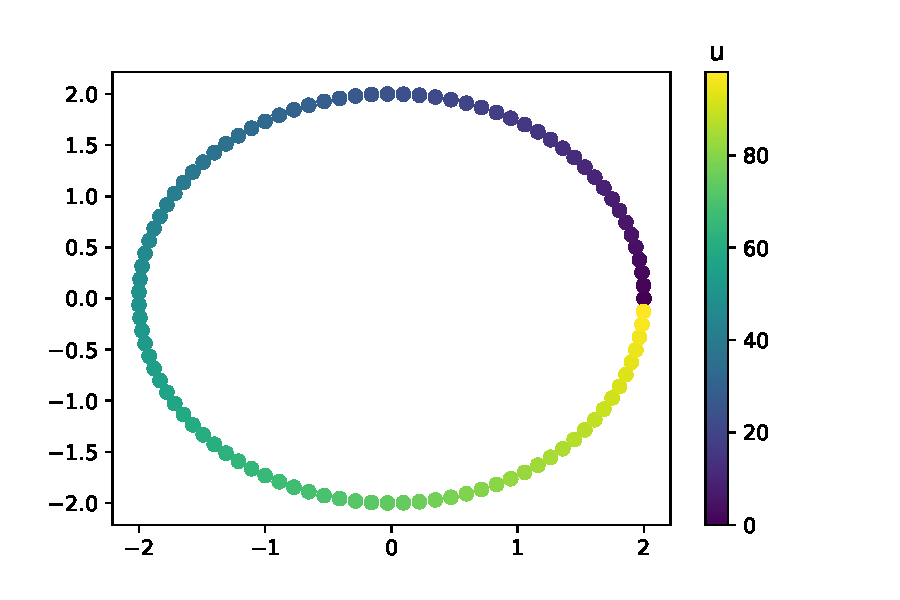
\includegraphics[scale=0.5]{./images/initial_conditons.pdf}
\end{figure}

\end{frame}

\begin{frame}{Solution}
\vspace{-0.5cm}
\begin{figure}
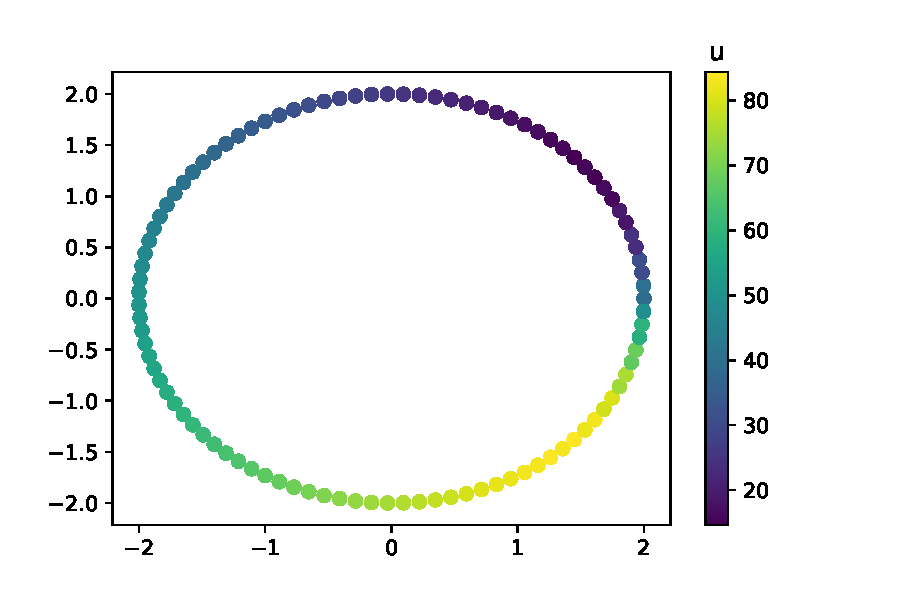
\includegraphics[scale=0.5]{./images/solution.pdf}
\end{figure}
\vspace{-0.5cm}
\begin{block}{Parameters}
\begin{itemize}
\item heat transfer coefficient $k$ = 0.5
\item time step size $dt$ = 1.;
\item grid spacing $h$ = 1.;
\item time steps $nt$ = 45;
\end{itemize}

\end{block}

\end{frame}

%%%%%%%%%%%%%%%%%%%%%%%%%%%%%%%%%%%%%%%%%%%%%%%%%%%%%%%%%%%%%%%%%%%%%%%%%%%%%%
\section{Summary}
%%%%%%%%%%%%%%%%%%%%%%%%%%%%%%%%%%%%%%%%%%%%%%%%%%%%%%%%%%%%%%%%%%%%%%%%%%%%%%
\begin{frame}{Summary}
\begin{block}{After this lecture, you should know}
\begin{itemize}
\item One-dimensional heat equation
\item Serial implementation
\end{itemize}
\end{block}
\end{frame}


%%%%%%%%%%%%%%%%%%%%%%%%%%%%%%%%%%%%%%%%%%%%%%%%%%%%%%%%%%%%%%%%%%%%%%%%%%%%%%
\section{References}
%%%%%%%%%%%%%%%%%%%%%%%%%%%%%%%%%%%%%%%%%%%%%%%%%%%%%%%%%%%%%%%%%%%%%%%%%%%%%%

\begin{frame}[t, allowframebreaks]
\frametitle{References}
\bibliographystyle{plain}
\bibliography{bib}
\end{frame}


\end{document}